\section{Entrepreneurial Intention Model}

\subsection{Ajzen's Theory of Planned Behavior}
%acronyms package reference: https://www.namsu.de/Extra/pakete/Acronym.html
The next paragraph is dedicated to the \acf{tpb}, which is the theoretical basis of our seminar paper. It was founded by Ajzen \cite{ajzen1991theory} and models the development of intent, which is considered a reliable predictor of behavior. \todo{some papers here}
\begin{figure}[h]
\begin{center}
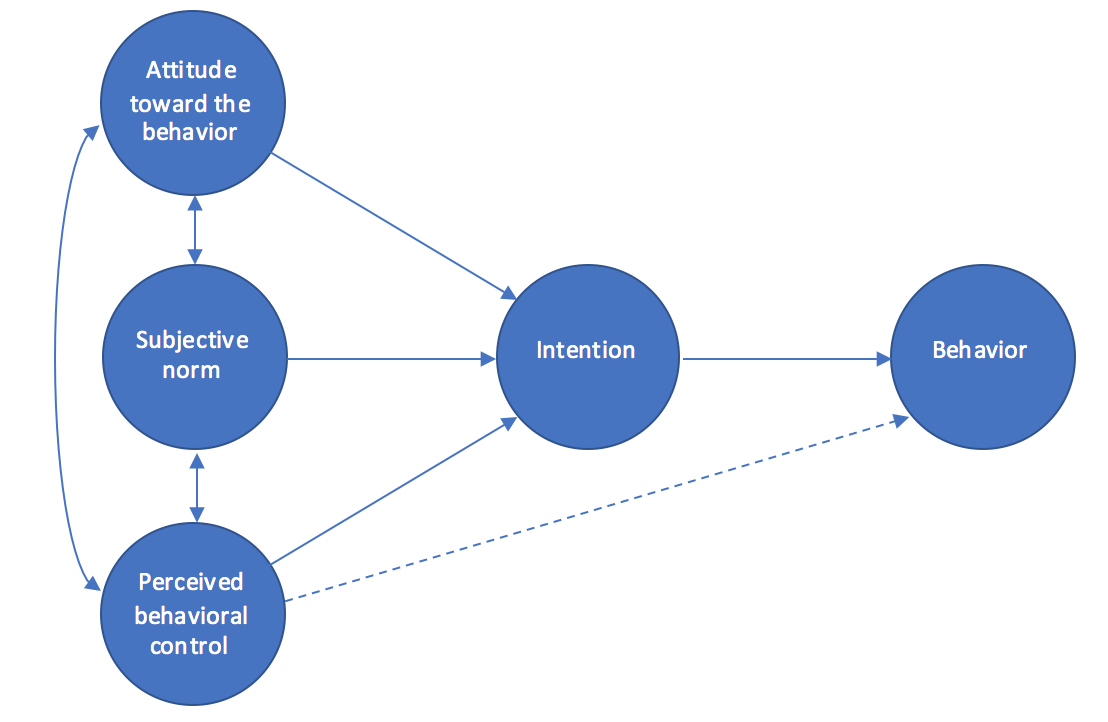
\includegraphics[width=13cm]{images/Ajzen.png}
\caption{Theory of Planned Behavior - Graphic according to Ajzen \cite{ajzen1991theory}}
\label{fig:Ajzen}
\end{center}
\end{figure}

According to the theory, intention has three antecedents: Attitude toward the behavior, subjective norm and perceived behavioral control (see Figure \ref{fig:Ajzen}). The components of \ac{tpb} are described in detail in the following paragraphs:

The central aspect of the \acf{tpb} are the intentions. They reflect a person's motivation and willingness to engage in effort to perform the behavior. Thus, the greater the intention, the more likely is the action. It is considered a good predictor of actual behavior (citations). While this relationship is quite natural and obvious, the question the TPB actually addresses is what influences the intention and how it can be predicted.

The first is the so called "perceived behavioral control": Ajzen states in his paper that the actual behavioral control as an influence factor is clear. An action that is not feasible due to resource, personal or other constraints, just cannot be pursued. That is why he focuses on the perception of behavioral control (PBC). Ajzen stresses, that PBC highly depends on the situation and is not a general perception of how optimistic a person is about their outcome depending on their action.

The second influence factor according to the \ac{tpb} are "subjective norms": The paper \cite{ajzen1991theory} states, that this antecedent of intentions reflects the social pressure imposed on an individual by others, i.e. family, friends and partners. This influence can either be positive or negative and therefore encourage or discourage the person to perform the action.\\
\hl{(what is the reasoning for choosing the antecedent?)}\\
\hl{(Ajzen also says, that this factor is minor, compared to the others, but let's have this in the criticism section)}

The last antecedent of intent is the "attitude towards the behavior": In the original paper about the \ac{tpb} (\cite{ajzen1991theory}), the attitude towards the behavior is described in a similar way as the social norms. It basically describes the personal opinion about the behavior, unlike social norms, which are the opinions of others.


\subsection{Criticism and Limitations of the \acl{tpb}}
Even though the \acl{tpb} is considered one of the most famous theories for entrepreneurial intent, there is still criticism about it. The following section features some of the criticism and limitations about this model.

The \ac{tpb} has the two antecedents "attitude towards the behavior" and "perceived behavioral control" which are accepted among many authors \todo{papers} but sometimes phrased in a different way.\\
"Attitude towards the behavior" is described as "perceived desirability" as they both enshrine the extent to which a person is favorable of or desires the action.
"Perceived behavioral control" is by some transcribed as "perceived self-efficacy"\\

Ajzen himself stated, that the antecedent "social norms" has limited impact compared to the other two influence factors of intentions. He concluded, that personal characteristics are stronger than the influence of others \cite{ajzen1991theory}. In fact, many authors neglect the "social norms" altogether in their study and only focus on \\

Another theory for modeling intentions and behaviors is Shapero's model of Entrepreneurial Event. It also incorporates perceived feasibility and perceived self-efficacy but has "" instead of social norms in \ac{tpb}.

One more recent study from Fitzsimmons and Douglas \cite{fitzsimmons2011interaction} covers the interaction between perceived desirability and perceived self-efficacy. According to their paper, either of those influence factors is sufficient to form entrepreneurial intent. If perceived desirability is high, adding perceived self-efficacy does not add much more to the score of intent. The same applies to high perceived self-efficacy and low desirability. This is in contrast to the \ac{tpb}. Fitzsimmons and Douglas refer to phenomenon in their paper as "natural entrepreneur" (high perceived desirability/high perceived self-efficacy), "accidental entrepreneur" (low/high) and "inevitable entrepreneur" (high/low).

%for example, that social norms have a limited impact
\begin{itemize}
\item Krueger 2000 - comparison with SEE; Social norms as an antecedent of IE may not be correct in TPB.
\item (Maybe) Shapero's model SEE
\item Fitzsimmons 2011 - negative interaction of perceived desirability and perceived feasibility
\end{itemize}


\begin{itemize}
\item Social norms with limited impact
\item SEE
\item PBC and attitudes towards the act are only other words for perceived desirability and perceived self-efficacy
\item Fitzsimmons 2011 finding, that only one of PD and PS are required to form intentions 
\end{itemize}

\todo{Limitations still missing}

\subsection{Why we still chose TBP (rephrase)}
We saw some of the limitations and criticism of \ac{tpb} in the previous section. That is why we are now to justify our choice of this model.
\todo{Lukas: @Kevin :*}
\textbf{Seite zwei in Fayolle (\cite{fayolle2015impact}) gibt gute punkte warum, ich nenne es auch schon twas in der einleitung}

\subsection{Further general findings about EI based on Ajzens Model}
As mentioned in the previous section, \ac{tpb} is popular in science. That is why there are many findings based on this theory. The following paragraph lists some of the most important findings based on \ac{tpb}.
%for example, that social norms have a limited impact
\begin{itemize}
\item Bullough, 2014, Importance of Self-efficacy and resiliance for EI
\item Fitzsimmons, Jason R.; Douglas, Evan J. (2011): Interaction between feasibility and desirability in the formation of entrepreneurial intentions
\item Krueger, Norris F.; Carsrud, Alan L. (1993): Entrepreneurial intentions. Applying the theory of planned behaviour
\item Linan, Francisco; Chen, Yi-Wen (2009): Development and Cross-Cultural Application of a Specific Instrument to Measure Entrepreneurial Intentions
\end{itemize}